\section{Árvores e Estruturas Derivadas}

\begin{frame}[plain]
  \centering
  \Huge \insertsection
\end{frame}

\begin{frame}{Árvore e Floresta}
  \centering
  \begin{itemize}
    \item \textbf{Árvore:} Grafo conexo, acíclico, com \(n\) vértices e \(n-1\) arestas.
    \item \textbf{Floresta:} Conjunto de árvores disjuntas.
  \end{itemize}

  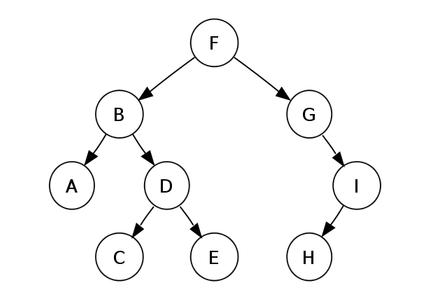
\includegraphics[width=0.5\textwidth]{./images/tree.png}

  \begin{block}{Propriedades}
    \begin{itemize}
      \item Exatamente um caminho entre dois nós.
      \item Remover uma aresta de uma árvore → floresta.
    \end{itemize}
  \end{block}
\end{frame}

\begin{frame}{Árvore Binária e Definições}
  \centering
  \begin{itemize}
    \item Cada nó possui no máximo 2 filhos: esquerdo e direito.
    \item \textbf{Raiz:} nó inicial.
    \item \textbf{Folha:} nó sem filhos.
    \item \textbf{Altura:} comprimento do caminho mais longo até uma folha.
    \item \textbf{Subárvore:} árvore contida dentro de outra.
  \end{itemize}
  
  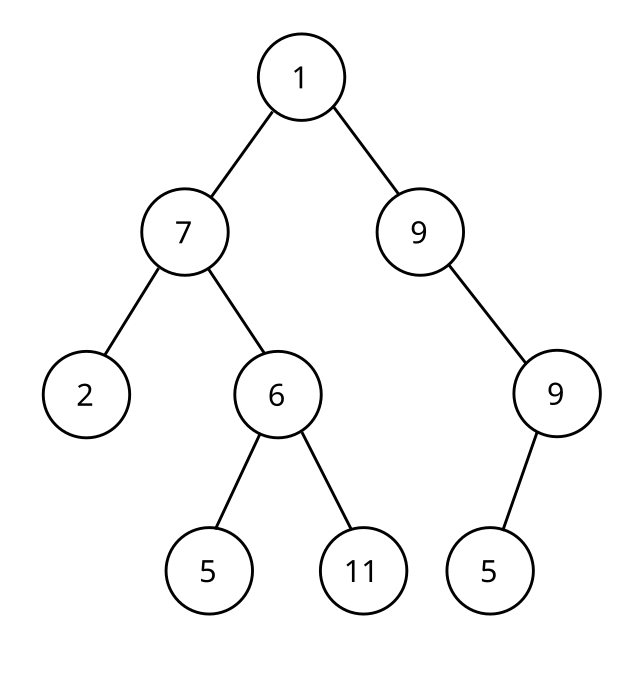
\includegraphics[width=0.5\textwidth]{./images/bintree.png}
\end{frame}

\begin{frame}{Árvore Ternária}
  \centering
  \begin{itemize}
    \item Cada nó pode ter até 3 filhos.
  \end{itemize}
  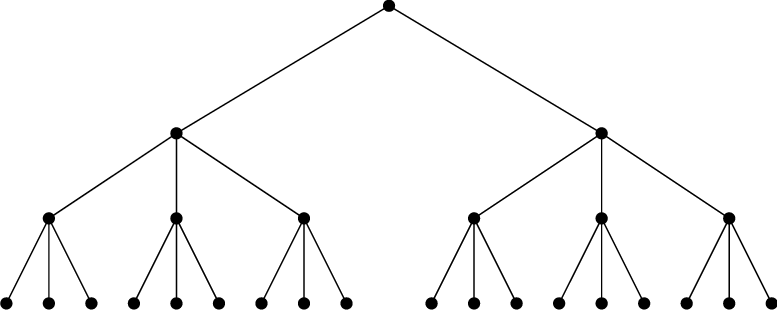
\includegraphics[width=1\textwidth]{./images/ttree.png}
\end{frame}

\begin{frame}{Aplicações de Árvores Binárias: Fibonacci}
  \centering
  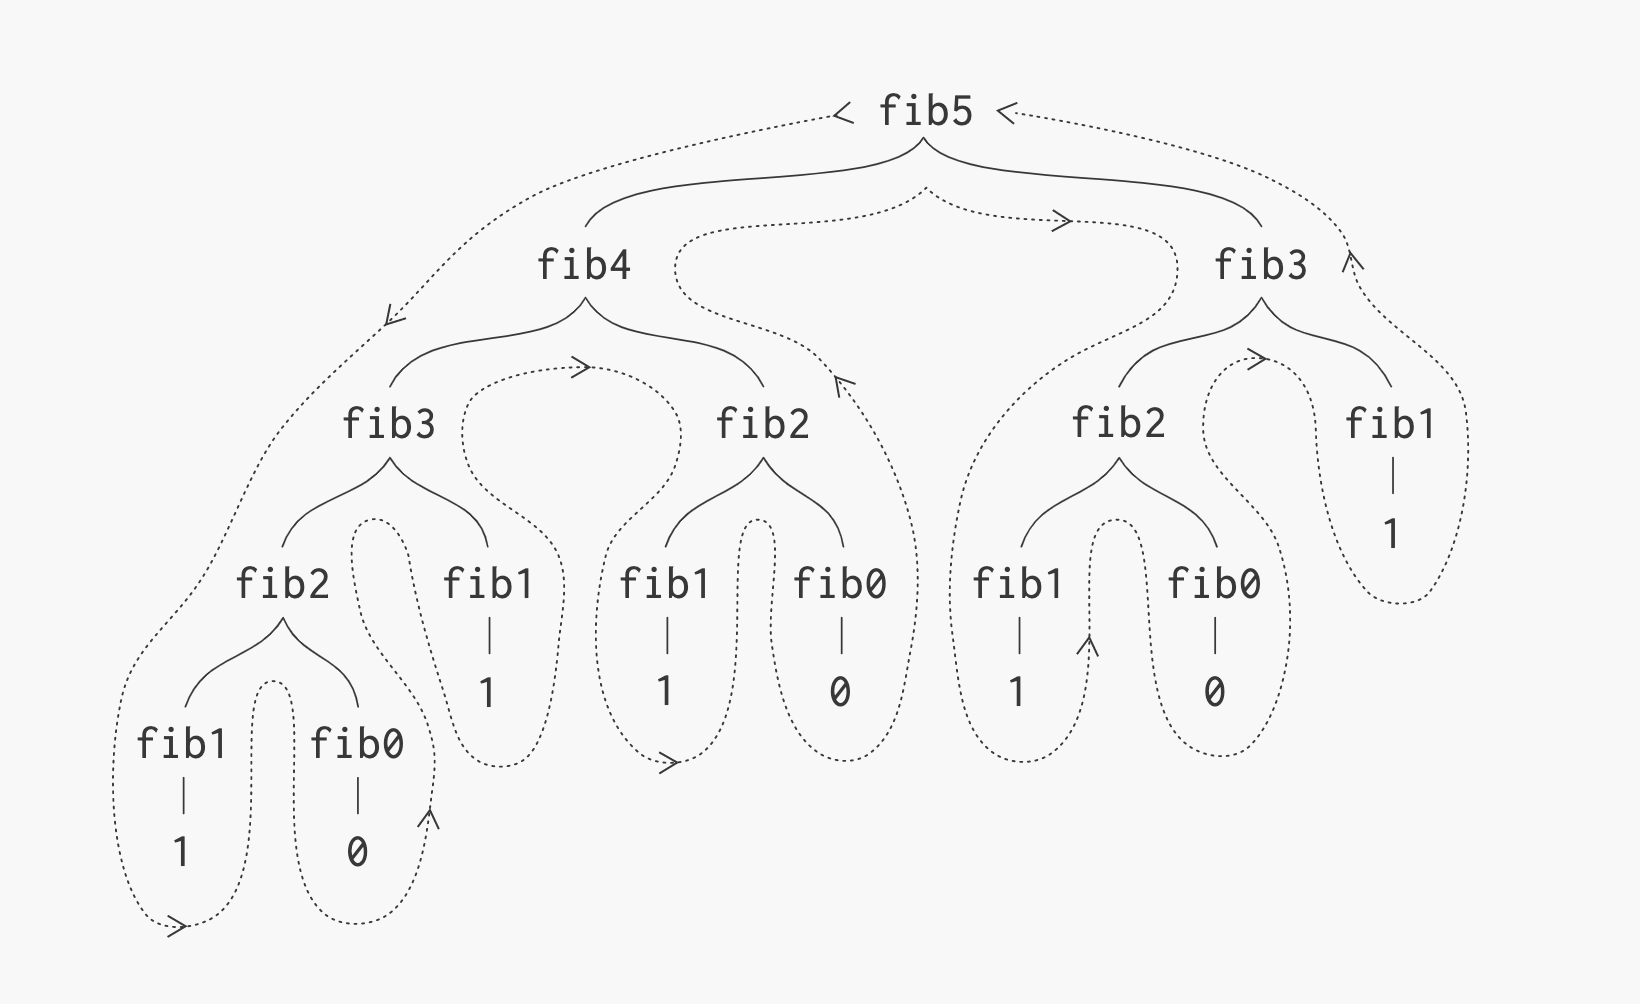
\includegraphics[width=1\textwidth]{./images/fib.png}
\end{frame}

\begin{frame}{Aplicações de Árvores Binárias: Quick Sort}
  \centering
  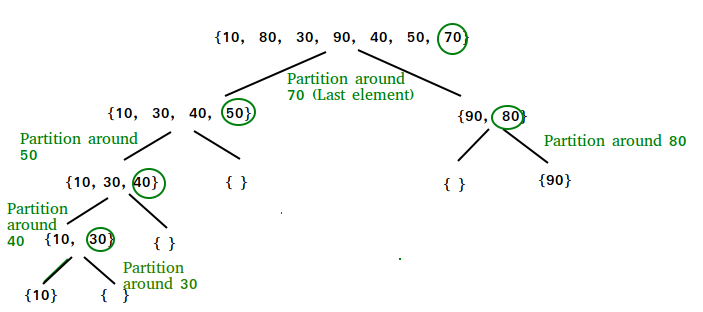
\includegraphics[width=1\textwidth]{./images/quick.png}
\end{frame}

\begin{frame}{Tipos de Árvores Binárias}
  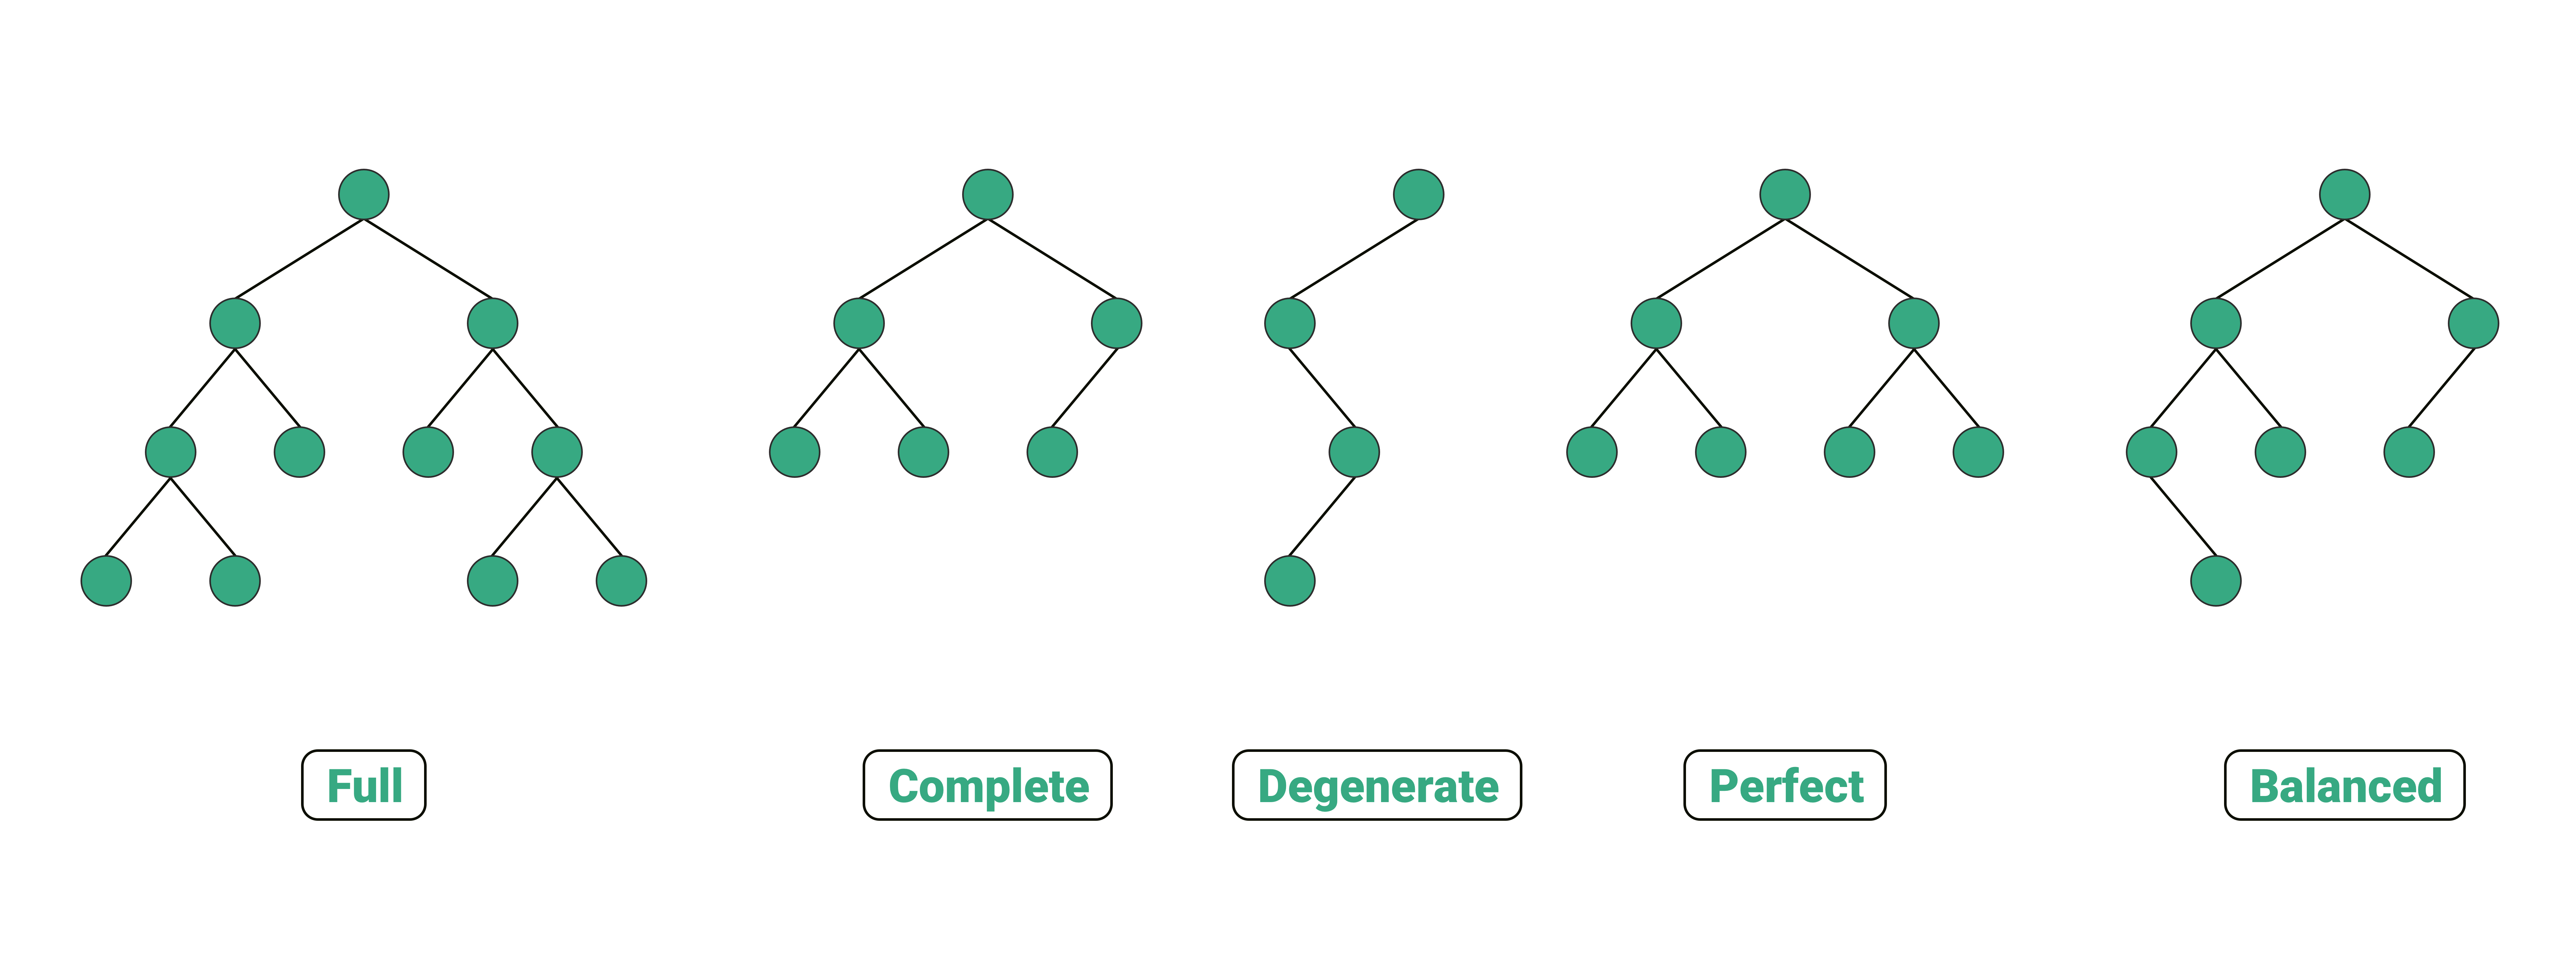
\includegraphics[width=1\textwidth]{./images/btreetypes.png}
\end{frame}

\begin{frame}{Árvore Binária de Busca (BST)}
  \centering
  \begin{itemize}
    \item Subárvore esquerda contém nós menores.
    \item Subárvore direita contém nós maiores.
    \item Operações típicas: busca, inserção, remoção → O(h)
  \end{itemize}

  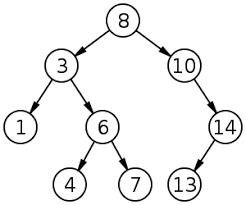
\includegraphics[width=0.75\textwidth]{./images/bst.png}

  \textit{Em árvores desbalanceadas, h pode chegar a n.}
\end{frame}

\begin{frame}{Árvore Rubro-Negra (Red-Black Tree)}
  \centering
  \begin{itemize}
    \item Árvore binária balanceada com regras de coloração.
    \item Altura mantida em O(log n).
    \item Rebalanceamento com rotações e trocas de cor.
    \item Muito usada em bibliotecas padrão (ex: `std::map` em C++).
  \end{itemize}
  
  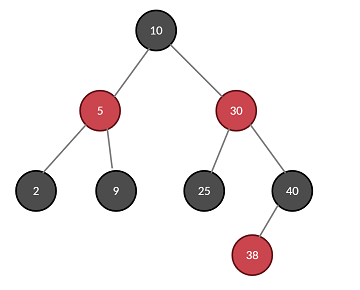
\includegraphics[width=0.75\textwidth]{./images/redblack.png}
\end{frame}

\begin{frame}{Árvore AVL}
  \centering
  \begin{itemize}
    \item Árvore binária de busca balanceada.
    \item Diferença entre alturas das subárvores de cada nó é no máximo 1.
    \item Requer rotações após inserções/remoções.
  \end{itemize}
  
  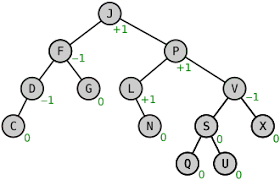
\includegraphics[width=0.75\textwidth]{./images/avl.png}
\end{frame}

\begin{frame}{Heap}
  \centering
  \begin{itemize}
    \item Estrutura de árvore quase completa.
    \item \textbf{Max-Heap:} pai $\geq$ filhos.
    \item \textbf{Min-Heap:} pai $\leq$ filhos.
    \item Usado em filas de prioridade.
  \end{itemize}
  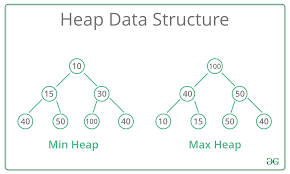
\includegraphics[width=0.75\textwidth]{./images/heaptt.png}
\end{frame}

\begin{frame}{Heap Sort}
  \centering
  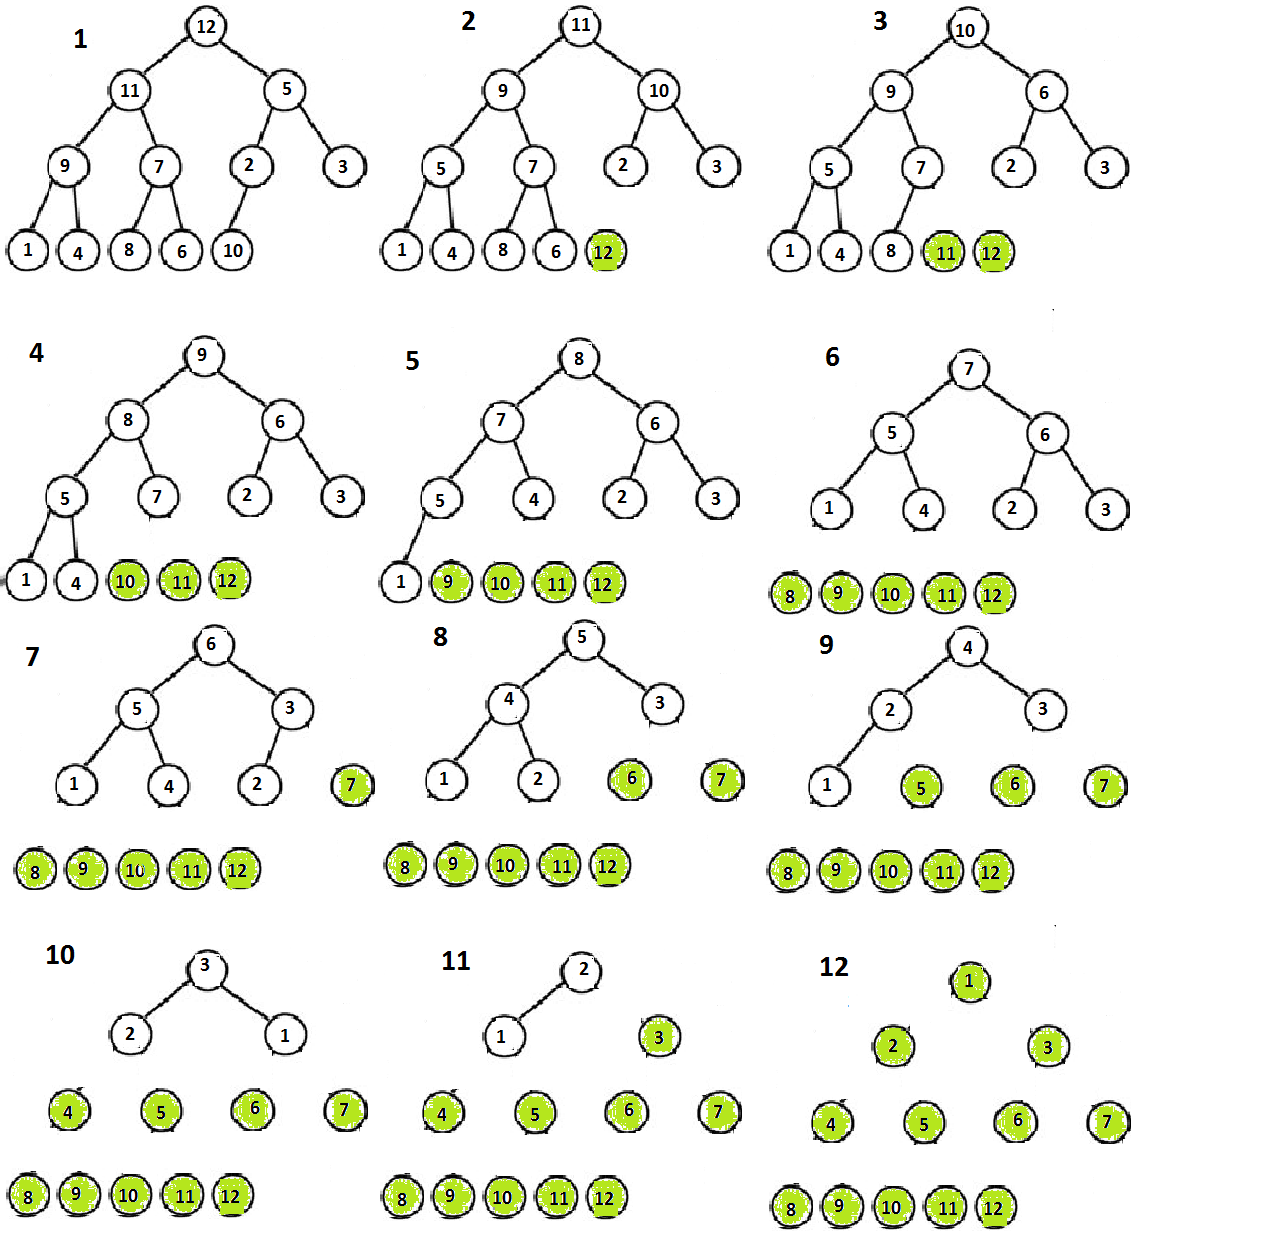
\includegraphics[width=0.75\textwidth]{./images/heaptree.png}
\end{frame}
